\chapter{DEPLOYMENT PLAN} 
With the completion of system testing and evaluation, we are now 
focusing on serving the system to the end users. This section will 
discuss the detailed deployment architecture and services. As we 
can see from Figure X, the proposed architecture contains the 
following components:
\begin{figure}[H]
    \centering
    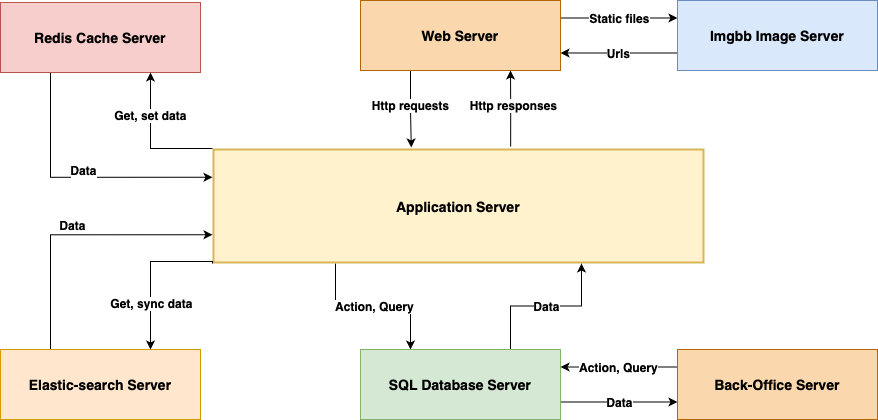
\includegraphics[width=0.9\textwidth]{Figures/Deployment/Pattern and Architecture-Deployment.drawio.png}
    \caption{Pattern and Architecture Deployment}
    \label{fig:deployment-architecture}
\end{figure}
The Web Server contains the Presentation layer of the system. It is the place that receives requests and sends 
back the web application or website to user browsers. It also 
handles user events and calls restful API from the Application 
Servers. A free Vercel cloud pipeline is used for this component.

The Application Servers contain the Business and Data Access layers 
of the system. This is the central part of the system, focusing on 
handling all business logic and flow, serving API for the web server, 
and interacting with other components of the system. We will use an Azure 
Virtual Machine to serve this component.

SQL Database Server is the place where the database of the system is served. 
This server interacts with the Application Server and Back-Office Server. 
This component will be deployed using an Azure SQL Database.

Imgbb Image Server stores all the static images of the system. Images will 
be uploaded directly from the Web Server to the Imgbb Image Server before 
storing the returned URLs in the SQL Database Server. This component will 
be served by a free Imgbb cloud service.

Finally, we will have two corresponding servers for caching data and optimizing 
data search speed using a free Elastic-search cloud and Azure Redis Cache Database.